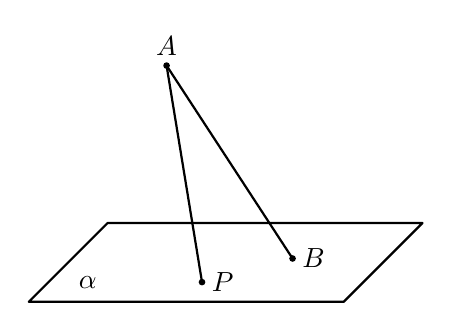
\begin{tikzpicture}[scale=1.0,line cap=round,line join=round]
\usetikzlibrary{calc}

% plane alpha as a parallelogram
\coordinate (L1) at (-2,0);
\coordinate (L2) at ( 2,0);
\coordinate (L3) at ( 3,1.0);
\coordinate (L4) at (-1,1.0);
\draw[thick] (L1)--(L2)--(L3)--(L4)--cycle;
\node at (-1.25,0.25) {$\alpha$};

% points on the plane
\coordinate (P) at (0.2,0.25);
\coordinate (B) at (1.35,0.55);
\fill (P) circle (1.2pt) node[right] {$P$};
\fill (B) circle (1.2pt) node[right] {$B$};

% point A above the plane
\coordinate (A) at (-0.25,3.0);
\fill (A) circle (1.2pt) node[above] {$A$};

% segments
\draw[thick] (A)--(B);
\draw[thick] (A)--(P);

\end{tikzpicture}